\section{Use Case: Click \& Ride App and Netzfahrplan}
\label{chap:useCases}
In this section, we describe the use cases which were used to proof that our approach for the automatic opitimized creation of railway timetables performes. 

\begin{itemize}
	\item[1)] Anwering a short-term train path request within three minutes
	\item[2)] Creating a timetable for one day 
\end{itemize}

\subsection{Click \& Ride App}
\label{chap:CnR}
For a short-term train path request, e.g. a train run for the next day, we can improve the response time to the railway operator by using our approach in a fully automated process. We will introduce the new way of booking a train path with a mobile application called "Click\&Ride-App". We commit to get the railway operator a train path offering within no longer than three minutes. In comparison, today's process for manual planning takes several hours or even up to three days. To ensure a maximum duration of three minutes we need to automazie every single step in the plannning process. A simplified process sequence is shown in figure \ref{fig:process_sequence}. 
\begin{figure}[htb]
	\centering
	% If you include a JPG file, 
	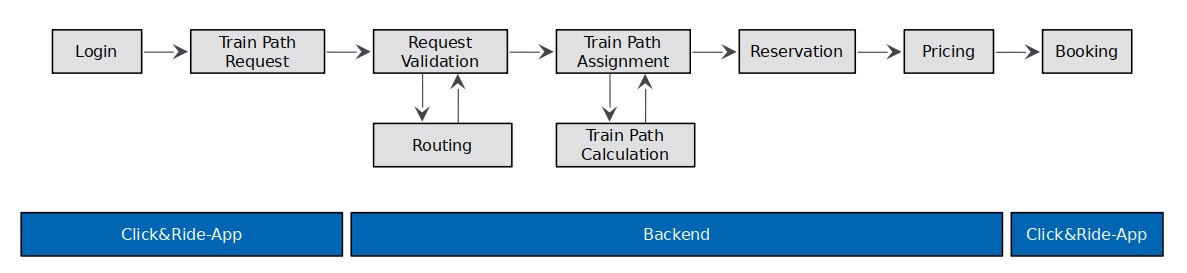
\includegraphics[width=\textwidth]{Bilder/process_sequence.jpg}
	% Else if you include an EPS file 
	%    (it may need an interpreter for the PostScript language, e.g. Ghostscript), 
	%\includegraphics[scale=0.30]{Fig1_Track.eps}
	\caption{Process of Click\&Ride}
	\label{fig:process_sequence}
\end{figure}

Click\&Ride is a new B2B channel so only railway operators may use the functionalities. After logging in, the the train path request will be submitted to the backend processes. At first there is a validation service that ensures formal and technical fit to the lines that will be used. For example an electric vehicle cannot use a line with no overhead line. If there are any problems with the train path request the railway operator gest instant feedback on the app's screen and can fix the problem.

\subsection{Netzfahrplan}
\label{chap:Netzfahrplan}
To create an automatic timetable for one day first you need to calculate the slots, where each slot starts and ends in one Betriebsstelle. Also every slot has up to three different train charakteristics and an amount of how many slots of which charakteristic are supposed to be produced. Those infomartion are necessary to preproduce a optimal set of slots with their most variety for the trainpath assignement.  \\
The second step is the train path assignment which needs the customer request. A customer request consist of the running points, time requirements and the characteristics of the train. The running points are at least the start of the request and its goal, but may also include some stops which should be served in between. The time requirements for our data consists only of an interval at the start of the request. But it is also possible to provide further time restrictions on the other running points. The characteristics of the request include all data necessary to calculate its dynamic properties such as acceleration and its static parameters like length, width and mass of the requested train.  \\
To discuss the solution of our process we created the slots for the european rail freight corridor one. Corridor one is the Rhine-Alpine Corridor stretches from sea ports of Rotterdam, Zeebrugge, Antwerp, Amsterdam and Vlissingen to the port of Genoa. During the course it passes five different countrys: Netherlands, Belgium, Germany, Switzerland and Italy. Here only the part in Germany Emmerich/Aachen to Basel will be considered. (see picture XXX). \\


%
\begin{table}[h]
	\centering
	\caption{Results for Netzfahrplan}
	\label{tab:result_Netzfpl}
	\begin{tabular}{lcccc} \hline
		\textbf{Text Style}   & \textbf{Font} & \textbf{Style} & \textbf{Size (pt)} \\ \hline
		Main text             & Times         & regular        & 10                 \\
		Section heading       & Times         & bold           & 12                 \\
		Subsection heading    & Times         & bold           & 10                 \\
		Subsubsection heading & Times         & bold           & 10                 \\ \hline
	\end{tabular}
\end{table}
\par


